\scanpage{19}\mspage{- IV- \handwritten{1102} -}
(21.6.5) Let us therefore consider a \uline{positive} divisor $D^{\unsure{\prime}}$ on $X$\inserted{ ($X$ be\deleted{\unsure{n}}ing assumed \uline{noetherian})}, so that the \inserted{fractional} Ideal $\underline I_{X}(D)$ is an \uline{Ideal of} $\underline O_{X}$, which is an \uline{invertible} $\underline O_{X}$-Module; let $Y(D)$ be the closed subprescheme of $X$ which it defines. \deleted{\unsure{This means}}\inserted{For} \deleted{\unsure{that}} every $x\handwritten{\in}Y(D)$, \deleted{\unsure{that,}} there is by hypothesis an \inserted{\handwritten{open}} neighborhood $U$ of $x$ in $X$ and a \uline{regular} section $t\handwritten{\in\Gamma}(U,\underline O_{X})$ such that $\underline I_{X}(D)\handwritten{\mid}U=\underline O_{U}\mathbin{.}t$ (21.2.7) ; in other words, the canonical immersion $Y(D)\handwritten{\to}X$ is \uline{regular and of codimension 1} \inserted{(19.1.4) at every point of $Y( D)$}. It will moreover be noted that conversely, if $Y$ \reversemarginpar
% slanted
\margin{\figure{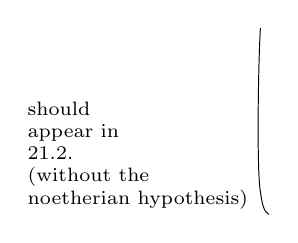
\begin{tikzpicture}[x=1em,y=1em,baseline=0pt]
  \node[anchor=north east,align=left,inner sep=0pt,font=\scriptsize] at (0,0)
    {\handwritten{should}\\
     \handwritten{appear in}\\
     \handwritten{21.2.}\\
     \handwritten{(without the}\\
     \handwritten{noetherian hypothesis)}};
  \draw[line width=.35pt] (.43,2.65) .. controls (.36,1.6) and (.29,-2.25) .. (.42,-3.2)
     .. controls (.49,-3.7) and (.55,-4) .. (.74,-4.08);
\end{tikzpicture}}}
is a closed subprescheme of $X$, regularly immersed in $X$ and \deleted{\unsure{is}} of codimension $1$ at every point of $Y$, there exists a positive divisor and only one \deleted{\unsure{positive}} $D$ on $X$ such that $Y(D)=Y$, because\deleted{\unsure{ this means}}\inserted{ for} \deleted{\unsure{that}} every $x\handwritten{\in}Y$, there is a neighborhood $U$ of $x$ in $X$ such that $Y\handwritten{\cap}U$ is defined by an Ideal of $\underline{\mathbb{O}}_{U}$ of the form $\underline O_{U}\mathbin{.}t$, where $t$ is \uline{regul\deleted{\unsure{re}}\handwritten{ar}} in $\handwritten{\Gamma}(U,\underline O_{X})$.


Since $X$ is assumed noetherian, $Y(D)$ has only a finite number of maximal points, and at each of these points $x$, we have $\operatorname{codim}(\handwritten{\{}x\handwritten{\}},X)={}\allowbreak{}=\operatorname{dim}(\underline O_{X,x})=1$, in other words $x\handwritten{\in}X^{(1)}$ ;
% slanted
\margin{\handwritten{\uline{reference} !}}\normalmarginpar
\deleted{\illegible{2} \unsure{part} \illegible{1}} moreover, $\underline O_{Y(D),x}$ is an \uline{artinian} ring at each of these poi\deleted{g}nts. At every point $x\handwritten{\in}X^{(1)}$ which is not a maximal point of $Y(D)$, we necessarily have $x\handwritten{\notin}Y(D)$, hence $\underline O_{Y(D),x}=0$. Put
\[
  \operatorname{cyc}(D)=\handwritten{\sum}^{\handwritten{\prime}}_{x\handwritten{\in}X^{(1)}}
  \operatorname{long}(\underline O_{Y(D),x})\mathbin{.}\handwritten{\overline}{\handwritten{\{}x\handwritten{\}}}
  \tag*{(21.6.5.1)}
\]
which is therefore an element of $Z^{1}(X)$.

\uline{Proposition} (21.6.6) .- \deleted{\uline{If} $X$ \uline{is noetherian}}, \uline{\deleted{t}\handwritten{T}he map} $D\handwritten{\leadsto}\operatorname{cyc}(D)$\deleted{\unsure{;}} \uline{is a homomorphism from the monoid} $\operatorname{Div}^{+}(X)$ \uline{to} $Z^{1}(X)$ .

It all comes down to seeing that for two \uline{positive} divisors $D,D'$, we have $\operatorname{cyc}(D+D')=\operatorname{cyc}(D)+\operatorname{cyc}(D')$. Now, we have (21.2.5) $\underline I_{X}(D+D')=\underline I_{X}(D)\underline I_{X}(D')$; it all comes down to seeing that if $x\handwritten{\in}X^{(1)}$, \inserted{\handwritten{if we put}} $A=\underline O_{X,x}$, and if $t$ and $t'$ are two regular elements of $A$, we have $\operatorname{long}(A/tt'A)=\operatorname{long}(A/tA)+{}\allowbreak{}+\operatorname{long}(A/t'A)$ ; but since \deleted{\unsure{$x$}} $t$ is regular, $tA/tt'A$ is isomorphic to $A/t'A$, whence \deleted{\unsure{follows}} immediately the proposition.

It follows immediately from the definitions that for every open subset $U\handwritten{\subset}X$, we
% archive sheet number: 18
